% Created by tikzDevice version 0.12
% !TEX encoding = UTF-8 Unicode
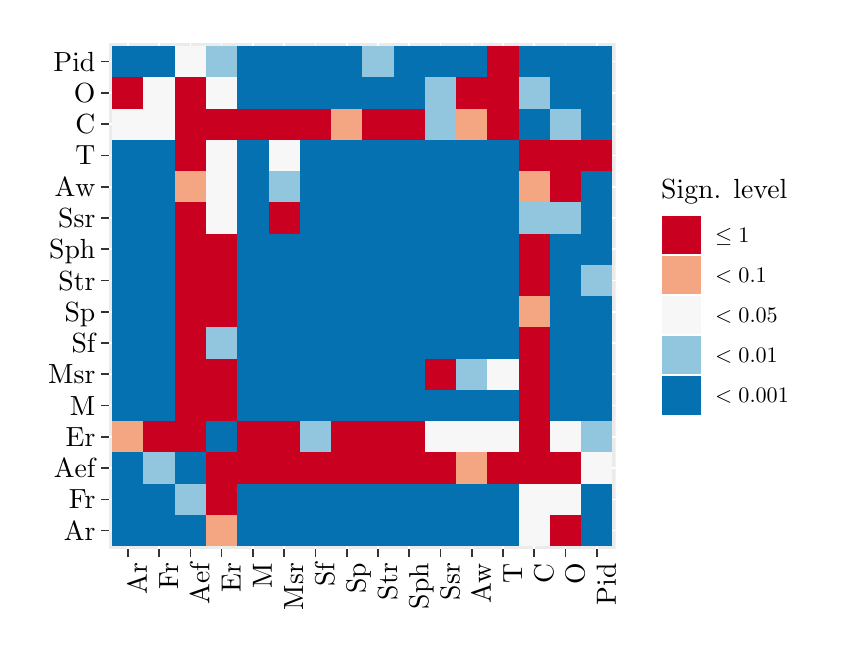
\begin{tikzpicture}[x=1pt,y=1pt]
\definecolor{fillColor}{RGB}{255,255,255}
\path[use as bounding box,fill=fillColor,fill opacity=0.00] (0,0) rectangle (288.00,216.00);
\begin{scope}
\path[clip] (  1.94,  0.00) rectangle (286.06,216.00);
\definecolor{drawColor}{RGB}{255,255,255}
\definecolor{fillColor}{RGB}{255,255,255}

\path[draw=drawColor,line width= 0.6pt,line join=round,line cap=round,fill=fillColor] (  1.94,  0.00) rectangle (286.06,216.00);
\end{scope}
\begin{scope}
\path[clip] ( 29.41, 27.47) rectangle (212.44,210.50);
\definecolor{fillColor}{gray}{0.92}

\path[fill=fillColor] ( 29.41, 27.47) rectangle (212.44,210.50);
\definecolor{drawColor}{RGB}{255,255,255}

\path[draw=drawColor,line width= 0.6pt,line join=round] ( 29.41, 34.25) --
	(212.44, 34.25);

\path[draw=drawColor,line width= 0.6pt,line join=round] ( 29.41, 45.55) --
	(212.44, 45.55);

\path[draw=drawColor,line width= 0.6pt,line join=round] ( 29.41, 56.85) --
	(212.44, 56.85);

\path[draw=drawColor,line width= 0.6pt,line join=round] ( 29.41, 68.15) --
	(212.44, 68.15);

\path[draw=drawColor,line width= 0.6pt,line join=round] ( 29.41, 79.44) --
	(212.44, 79.44);

\path[draw=drawColor,line width= 0.6pt,line join=round] ( 29.41, 90.74) --
	(212.44, 90.74);

\path[draw=drawColor,line width= 0.6pt,line join=round] ( 29.41,102.04) --
	(212.44,102.04);

\path[draw=drawColor,line width= 0.6pt,line join=round] ( 29.41,113.34) --
	(212.44,113.34);

\path[draw=drawColor,line width= 0.6pt,line join=round] ( 29.41,124.64) --
	(212.44,124.64);

\path[draw=drawColor,line width= 0.6pt,line join=round] ( 29.41,135.93) --
	(212.44,135.93);

\path[draw=drawColor,line width= 0.6pt,line join=round] ( 29.41,147.23) --
	(212.44,147.23);

\path[draw=drawColor,line width= 0.6pt,line join=round] ( 29.41,158.53) --
	(212.44,158.53);

\path[draw=drawColor,line width= 0.6pt,line join=round] ( 29.41,169.83) --
	(212.44,169.83);

\path[draw=drawColor,line width= 0.6pt,line join=round] ( 29.41,181.13) --
	(212.44,181.13);

\path[draw=drawColor,line width= 0.6pt,line join=round] ( 29.41,192.42) --
	(212.44,192.42);

\path[draw=drawColor,line width= 0.6pt,line join=round] ( 29.41,203.72) --
	(212.44,203.72);

\path[draw=drawColor,line width= 0.6pt,line join=round] ( 36.19, 27.47) --
	( 36.19,210.50);

\path[draw=drawColor,line width= 0.6pt,line join=round] ( 47.49, 27.47) --
	( 47.49,210.50);

\path[draw=drawColor,line width= 0.6pt,line join=round] ( 58.79, 27.47) --
	( 58.79,210.50);

\path[draw=drawColor,line width= 0.6pt,line join=round] ( 70.09, 27.47) --
	( 70.09,210.50);

\path[draw=drawColor,line width= 0.6pt,line join=round] ( 81.38, 27.47) --
	( 81.38,210.50);

\path[draw=drawColor,line width= 0.6pt,line join=round] ( 92.68, 27.47) --
	( 92.68,210.50);

\path[draw=drawColor,line width= 0.6pt,line join=round] (103.98, 27.47) --
	(103.98,210.50);

\path[draw=drawColor,line width= 0.6pt,line join=round] (115.28, 27.47) --
	(115.28,210.50);

\path[draw=drawColor,line width= 0.6pt,line join=round] (126.58, 27.47) --
	(126.58,210.50);

\path[draw=drawColor,line width= 0.6pt,line join=round] (137.87, 27.47) --
	(137.87,210.50);

\path[draw=drawColor,line width= 0.6pt,line join=round] (149.17, 27.47) --
	(149.17,210.50);

\path[draw=drawColor,line width= 0.6pt,line join=round] (160.47, 27.47) --
	(160.47,210.50);

\path[draw=drawColor,line width= 0.6pt,line join=round] (171.77, 27.47) --
	(171.77,210.50);

\path[draw=drawColor,line width= 0.6pt,line join=round] (183.07, 27.47) --
	(183.07,210.50);

\path[draw=drawColor,line width= 0.6pt,line join=round] (194.36, 27.47) --
	(194.36,210.50);

\path[draw=drawColor,line width= 0.6pt,line join=round] (205.66, 27.47) --
	(205.66,210.50);
\definecolor{fillColor}{RGB}{5,113,176}

\path[fill=fillColor] ( 30.54, 28.60) rectangle ( 41.84, 39.90);

\path[fill=fillColor] ( 41.84, 28.60) rectangle ( 53.14, 39.90);

\path[fill=fillColor] ( 53.14, 28.60) rectangle ( 64.44, 39.90);
\definecolor{fillColor}{RGB}{244,165,130}

\path[fill=fillColor] ( 64.44, 28.60) rectangle ( 75.73, 39.90);
\definecolor{fillColor}{RGB}{5,113,176}

\path[fill=fillColor] ( 75.73, 28.60) rectangle ( 87.03, 39.90);

\path[fill=fillColor] ( 87.03, 28.60) rectangle ( 98.33, 39.90);

\path[fill=fillColor] ( 98.33, 28.60) rectangle (109.63, 39.90);

\path[fill=fillColor] (109.63, 28.60) rectangle (120.93, 39.90);

\path[fill=fillColor] (120.93, 28.60) rectangle (132.22, 39.90);

\path[fill=fillColor] (132.22, 28.60) rectangle (143.52, 39.90);

\path[fill=fillColor] (143.52, 28.60) rectangle (154.82, 39.90);

\path[fill=fillColor] (154.82, 28.60) rectangle (166.12, 39.90);

\path[fill=fillColor] (166.12, 28.60) rectangle (177.42, 39.90);
\definecolor{fillColor}{gray}{0.97}

\path[fill=fillColor] (177.42, 28.60) rectangle (188.71, 39.90);
\definecolor{fillColor}{RGB}{202,0,32}

\path[fill=fillColor] (188.71, 28.60) rectangle (200.01, 39.90);
\definecolor{fillColor}{RGB}{5,113,176}

\path[fill=fillColor] (200.01, 28.60) rectangle (211.31, 39.90);

\path[fill=fillColor] ( 30.54, 39.90) rectangle ( 41.84, 51.20);

\path[fill=fillColor] ( 41.84, 39.90) rectangle ( 53.14, 51.20);
\definecolor{fillColor}{RGB}{146,197,222}

\path[fill=fillColor] ( 53.14, 39.90) rectangle ( 64.44, 51.20);
\definecolor{fillColor}{RGB}{202,0,32}

\path[fill=fillColor] ( 64.44, 39.90) rectangle ( 75.73, 51.20);
\definecolor{fillColor}{RGB}{5,113,176}

\path[fill=fillColor] ( 75.73, 39.90) rectangle ( 87.03, 51.20);

\path[fill=fillColor] ( 87.03, 39.90) rectangle ( 98.33, 51.20);

\path[fill=fillColor] ( 98.33, 39.90) rectangle (109.63, 51.20);

\path[fill=fillColor] (109.63, 39.90) rectangle (120.93, 51.20);

\path[fill=fillColor] (120.93, 39.90) rectangle (132.22, 51.20);

\path[fill=fillColor] (132.22, 39.90) rectangle (143.52, 51.20);

\path[fill=fillColor] (143.52, 39.90) rectangle (154.82, 51.20);

\path[fill=fillColor] (154.82, 39.90) rectangle (166.12, 51.20);

\path[fill=fillColor] (166.12, 39.90) rectangle (177.42, 51.20);
\definecolor{fillColor}{gray}{0.97}

\path[fill=fillColor] (177.42, 39.90) rectangle (188.71, 51.20);

\path[fill=fillColor] (188.71, 39.90) rectangle (200.01, 51.20);
\definecolor{fillColor}{RGB}{5,113,176}

\path[fill=fillColor] (200.01, 39.90) rectangle (211.31, 51.20);

\path[fill=fillColor] ( 30.54, 51.20) rectangle ( 41.84, 62.50);
\definecolor{fillColor}{RGB}{146,197,222}

\path[fill=fillColor] ( 41.84, 51.20) rectangle ( 53.14, 62.50);
\definecolor{fillColor}{RGB}{5,113,176}

\path[fill=fillColor] ( 53.14, 51.20) rectangle ( 64.44, 62.50);
\definecolor{fillColor}{RGB}{202,0,32}

\path[fill=fillColor] ( 64.44, 51.20) rectangle ( 75.73, 62.50);

\path[fill=fillColor] ( 75.73, 51.20) rectangle ( 87.03, 62.50);

\path[fill=fillColor] ( 87.03, 51.20) rectangle ( 98.33, 62.50);

\path[fill=fillColor] ( 98.33, 51.20) rectangle (109.63, 62.50);

\path[fill=fillColor] (109.63, 51.20) rectangle (120.93, 62.50);

\path[fill=fillColor] (120.93, 51.20) rectangle (132.22, 62.50);

\path[fill=fillColor] (132.22, 51.20) rectangle (143.52, 62.50);

\path[fill=fillColor] (143.52, 51.20) rectangle (154.82, 62.50);
\definecolor{fillColor}{RGB}{244,165,130}

\path[fill=fillColor] (154.82, 51.20) rectangle (166.12, 62.50);
\definecolor{fillColor}{RGB}{202,0,32}

\path[fill=fillColor] (166.12, 51.20) rectangle (177.42, 62.50);

\path[fill=fillColor] (177.42, 51.20) rectangle (188.71, 62.50);

\path[fill=fillColor] (188.71, 51.20) rectangle (200.01, 62.50);
\definecolor{fillColor}{gray}{0.97}

\path[fill=fillColor] (200.01, 51.20) rectangle (211.31, 62.50);
\definecolor{fillColor}{RGB}{244,165,130}

\path[fill=fillColor] ( 30.54, 62.50) rectangle ( 41.84, 73.80);
\definecolor{fillColor}{RGB}{202,0,32}

\path[fill=fillColor] ( 41.84, 62.50) rectangle ( 53.14, 73.80);

\path[fill=fillColor] ( 53.14, 62.50) rectangle ( 64.44, 73.80);
\definecolor{fillColor}{RGB}{5,113,176}

\path[fill=fillColor] ( 64.44, 62.50) rectangle ( 75.73, 73.80);
\definecolor{fillColor}{RGB}{202,0,32}

\path[fill=fillColor] ( 75.73, 62.50) rectangle ( 87.03, 73.80);

\path[fill=fillColor] ( 87.03, 62.50) rectangle ( 98.33, 73.80);
\definecolor{fillColor}{RGB}{146,197,222}

\path[fill=fillColor] ( 98.33, 62.50) rectangle (109.63, 73.80);
\definecolor{fillColor}{RGB}{202,0,32}

\path[fill=fillColor] (109.63, 62.50) rectangle (120.93, 73.80);

\path[fill=fillColor] (120.93, 62.50) rectangle (132.22, 73.80);

\path[fill=fillColor] (132.22, 62.50) rectangle (143.52, 73.80);
\definecolor{fillColor}{gray}{0.97}

\path[fill=fillColor] (143.52, 62.50) rectangle (154.82, 73.80);

\path[fill=fillColor] (154.82, 62.50) rectangle (166.12, 73.80);

\path[fill=fillColor] (166.12, 62.50) rectangle (177.42, 73.80);
\definecolor{fillColor}{RGB}{202,0,32}

\path[fill=fillColor] (177.42, 62.50) rectangle (188.71, 73.80);
\definecolor{fillColor}{gray}{0.97}

\path[fill=fillColor] (188.71, 62.50) rectangle (200.01, 73.80);
\definecolor{fillColor}{RGB}{146,197,222}

\path[fill=fillColor] (200.01, 62.50) rectangle (211.31, 73.80);
\definecolor{fillColor}{RGB}{5,113,176}

\path[fill=fillColor] ( 30.54, 73.80) rectangle ( 41.84, 85.09);

\path[fill=fillColor] ( 41.84, 73.80) rectangle ( 53.14, 85.09);
\definecolor{fillColor}{RGB}{202,0,32}

\path[fill=fillColor] ( 53.14, 73.80) rectangle ( 64.44, 85.09);

\path[fill=fillColor] ( 64.44, 73.80) rectangle ( 75.73, 85.09);
\definecolor{fillColor}{RGB}{5,113,176}

\path[fill=fillColor] ( 75.73, 73.80) rectangle ( 87.03, 85.09);

\path[fill=fillColor] ( 87.03, 73.80) rectangle ( 98.33, 85.09);

\path[fill=fillColor] ( 98.33, 73.80) rectangle (109.63, 85.09);

\path[fill=fillColor] (109.63, 73.80) rectangle (120.93, 85.09);

\path[fill=fillColor] (120.93, 73.80) rectangle (132.22, 85.09);

\path[fill=fillColor] (132.22, 73.80) rectangle (143.52, 85.09);

\path[fill=fillColor] (143.52, 73.80) rectangle (154.82, 85.09);

\path[fill=fillColor] (154.82, 73.80) rectangle (166.12, 85.09);

\path[fill=fillColor] (166.12, 73.80) rectangle (177.42, 85.09);
\definecolor{fillColor}{RGB}{202,0,32}

\path[fill=fillColor] (177.42, 73.80) rectangle (188.71, 85.09);
\definecolor{fillColor}{RGB}{5,113,176}

\path[fill=fillColor] (188.71, 73.80) rectangle (200.01, 85.09);

\path[fill=fillColor] (200.01, 73.80) rectangle (211.31, 85.09);

\path[fill=fillColor] ( 30.54, 85.09) rectangle ( 41.84, 96.39);

\path[fill=fillColor] ( 41.84, 85.09) rectangle ( 53.14, 96.39);
\definecolor{fillColor}{RGB}{202,0,32}

\path[fill=fillColor] ( 53.14, 85.09) rectangle ( 64.44, 96.39);

\path[fill=fillColor] ( 64.44, 85.09) rectangle ( 75.73, 96.39);
\definecolor{fillColor}{RGB}{5,113,176}

\path[fill=fillColor] ( 75.73, 85.09) rectangle ( 87.03, 96.39);

\path[fill=fillColor] ( 87.03, 85.09) rectangle ( 98.33, 96.39);

\path[fill=fillColor] ( 98.33, 85.09) rectangle (109.63, 96.39);

\path[fill=fillColor] (109.63, 85.09) rectangle (120.93, 96.39);

\path[fill=fillColor] (120.93, 85.09) rectangle (132.22, 96.39);

\path[fill=fillColor] (132.22, 85.09) rectangle (143.52, 96.39);
\definecolor{fillColor}{RGB}{202,0,32}

\path[fill=fillColor] (143.52, 85.09) rectangle (154.82, 96.39);
\definecolor{fillColor}{RGB}{146,197,222}

\path[fill=fillColor] (154.82, 85.09) rectangle (166.12, 96.39);
\definecolor{fillColor}{gray}{0.97}

\path[fill=fillColor] (166.12, 85.09) rectangle (177.42, 96.39);
\definecolor{fillColor}{RGB}{202,0,32}

\path[fill=fillColor] (177.42, 85.09) rectangle (188.71, 96.39);
\definecolor{fillColor}{RGB}{5,113,176}

\path[fill=fillColor] (188.71, 85.09) rectangle (200.01, 96.39);

\path[fill=fillColor] (200.01, 85.09) rectangle (211.31, 96.39);

\path[fill=fillColor] ( 30.54, 96.39) rectangle ( 41.84,107.69);

\path[fill=fillColor] ( 41.84, 96.39) rectangle ( 53.14,107.69);
\definecolor{fillColor}{RGB}{202,0,32}

\path[fill=fillColor] ( 53.14, 96.39) rectangle ( 64.44,107.69);
\definecolor{fillColor}{RGB}{146,197,222}

\path[fill=fillColor] ( 64.44, 96.39) rectangle ( 75.73,107.69);
\definecolor{fillColor}{RGB}{5,113,176}

\path[fill=fillColor] ( 75.73, 96.39) rectangle ( 87.03,107.69);

\path[fill=fillColor] ( 87.03, 96.39) rectangle ( 98.33,107.69);

\path[fill=fillColor] ( 98.33, 96.39) rectangle (109.63,107.69);

\path[fill=fillColor] (109.63, 96.39) rectangle (120.93,107.69);

\path[fill=fillColor] (120.93, 96.39) rectangle (132.22,107.69);

\path[fill=fillColor] (132.22, 96.39) rectangle (143.52,107.69);

\path[fill=fillColor] (143.52, 96.39) rectangle (154.82,107.69);

\path[fill=fillColor] (154.82, 96.39) rectangle (166.12,107.69);

\path[fill=fillColor] (166.12, 96.39) rectangle (177.42,107.69);
\definecolor{fillColor}{RGB}{202,0,32}

\path[fill=fillColor] (177.42, 96.39) rectangle (188.71,107.69);
\definecolor{fillColor}{RGB}{5,113,176}

\path[fill=fillColor] (188.71, 96.39) rectangle (200.01,107.69);

\path[fill=fillColor] (200.01, 96.39) rectangle (211.31,107.69);

\path[fill=fillColor] ( 30.54,107.69) rectangle ( 41.84,118.99);

\path[fill=fillColor] ( 41.84,107.69) rectangle ( 53.14,118.99);
\definecolor{fillColor}{RGB}{202,0,32}

\path[fill=fillColor] ( 53.14,107.69) rectangle ( 64.44,118.99);

\path[fill=fillColor] ( 64.44,107.69) rectangle ( 75.73,118.99);
\definecolor{fillColor}{RGB}{5,113,176}

\path[fill=fillColor] ( 75.73,107.69) rectangle ( 87.03,118.99);

\path[fill=fillColor] ( 87.03,107.69) rectangle ( 98.33,118.99);

\path[fill=fillColor] ( 98.33,107.69) rectangle (109.63,118.99);

\path[fill=fillColor] (109.63,107.69) rectangle (120.93,118.99);

\path[fill=fillColor] (120.93,107.69) rectangle (132.22,118.99);

\path[fill=fillColor] (132.22,107.69) rectangle (143.52,118.99);

\path[fill=fillColor] (143.52,107.69) rectangle (154.82,118.99);

\path[fill=fillColor] (154.82,107.69) rectangle (166.12,118.99);

\path[fill=fillColor] (166.12,107.69) rectangle (177.42,118.99);
\definecolor{fillColor}{RGB}{244,165,130}

\path[fill=fillColor] (177.42,107.69) rectangle (188.71,118.99);
\definecolor{fillColor}{RGB}{5,113,176}

\path[fill=fillColor] (188.71,107.69) rectangle (200.01,118.99);

\path[fill=fillColor] (200.01,107.69) rectangle (211.31,118.99);

\path[fill=fillColor] ( 30.54,118.99) rectangle ( 41.84,130.28);

\path[fill=fillColor] ( 41.84,118.99) rectangle ( 53.14,130.28);
\definecolor{fillColor}{RGB}{202,0,32}

\path[fill=fillColor] ( 53.14,118.99) rectangle ( 64.44,130.28);

\path[fill=fillColor] ( 64.44,118.99) rectangle ( 75.73,130.28);
\definecolor{fillColor}{RGB}{5,113,176}

\path[fill=fillColor] ( 75.73,118.99) rectangle ( 87.03,130.28);

\path[fill=fillColor] ( 87.03,118.99) rectangle ( 98.33,130.28);

\path[fill=fillColor] ( 98.33,118.99) rectangle (109.63,130.28);

\path[fill=fillColor] (109.63,118.99) rectangle (120.93,130.28);

\path[fill=fillColor] (120.93,118.99) rectangle (132.22,130.28);

\path[fill=fillColor] (132.22,118.99) rectangle (143.52,130.28);

\path[fill=fillColor] (143.52,118.99) rectangle (154.82,130.28);

\path[fill=fillColor] (154.82,118.99) rectangle (166.12,130.28);

\path[fill=fillColor] (166.12,118.99) rectangle (177.42,130.28);
\definecolor{fillColor}{RGB}{202,0,32}

\path[fill=fillColor] (177.42,118.99) rectangle (188.71,130.28);
\definecolor{fillColor}{RGB}{5,113,176}

\path[fill=fillColor] (188.71,118.99) rectangle (200.01,130.28);
\definecolor{fillColor}{RGB}{146,197,222}

\path[fill=fillColor] (200.01,118.99) rectangle (211.31,130.28);
\definecolor{fillColor}{RGB}{5,113,176}

\path[fill=fillColor] ( 30.54,130.28) rectangle ( 41.84,141.58);

\path[fill=fillColor] ( 41.84,130.28) rectangle ( 53.14,141.58);
\definecolor{fillColor}{RGB}{202,0,32}

\path[fill=fillColor] ( 53.14,130.28) rectangle ( 64.44,141.58);

\path[fill=fillColor] ( 64.44,130.28) rectangle ( 75.73,141.58);
\definecolor{fillColor}{RGB}{5,113,176}

\path[fill=fillColor] ( 75.73,130.28) rectangle ( 87.03,141.58);

\path[fill=fillColor] ( 87.03,130.28) rectangle ( 98.33,141.58);

\path[fill=fillColor] ( 98.33,130.28) rectangle (109.63,141.58);

\path[fill=fillColor] (109.63,130.28) rectangle (120.93,141.58);

\path[fill=fillColor] (120.93,130.28) rectangle (132.22,141.58);

\path[fill=fillColor] (132.22,130.28) rectangle (143.52,141.58);

\path[fill=fillColor] (143.52,130.28) rectangle (154.82,141.58);

\path[fill=fillColor] (154.82,130.28) rectangle (166.12,141.58);

\path[fill=fillColor] (166.12,130.28) rectangle (177.42,141.58);
\definecolor{fillColor}{RGB}{202,0,32}

\path[fill=fillColor] (177.42,130.28) rectangle (188.71,141.58);
\definecolor{fillColor}{RGB}{5,113,176}

\path[fill=fillColor] (188.71,130.28) rectangle (200.01,141.58);

\path[fill=fillColor] (200.01,130.28) rectangle (211.31,141.58);

\path[fill=fillColor] ( 30.54,141.58) rectangle ( 41.84,152.88);

\path[fill=fillColor] ( 41.84,141.58) rectangle ( 53.14,152.88);
\definecolor{fillColor}{RGB}{202,0,32}

\path[fill=fillColor] ( 53.14,141.58) rectangle ( 64.44,152.88);
\definecolor{fillColor}{gray}{0.97}

\path[fill=fillColor] ( 64.44,141.58) rectangle ( 75.73,152.88);
\definecolor{fillColor}{RGB}{5,113,176}

\path[fill=fillColor] ( 75.73,141.58) rectangle ( 87.03,152.88);
\definecolor{fillColor}{RGB}{202,0,32}

\path[fill=fillColor] ( 87.03,141.58) rectangle ( 98.33,152.88);
\definecolor{fillColor}{RGB}{5,113,176}

\path[fill=fillColor] ( 98.33,141.58) rectangle (109.63,152.88);

\path[fill=fillColor] (109.63,141.58) rectangle (120.93,152.88);

\path[fill=fillColor] (120.93,141.58) rectangle (132.22,152.88);

\path[fill=fillColor] (132.22,141.58) rectangle (143.52,152.88);

\path[fill=fillColor] (143.52,141.58) rectangle (154.82,152.88);

\path[fill=fillColor] (154.82,141.58) rectangle (166.12,152.88);

\path[fill=fillColor] (166.12,141.58) rectangle (177.42,152.88);
\definecolor{fillColor}{RGB}{146,197,222}

\path[fill=fillColor] (177.42,141.58) rectangle (188.71,152.88);

\path[fill=fillColor] (188.71,141.58) rectangle (200.01,152.88);
\definecolor{fillColor}{RGB}{5,113,176}

\path[fill=fillColor] (200.01,141.58) rectangle (211.31,152.88);

\path[fill=fillColor] ( 30.54,152.88) rectangle ( 41.84,164.18);

\path[fill=fillColor] ( 41.84,152.88) rectangle ( 53.14,164.18);
\definecolor{fillColor}{RGB}{244,165,130}

\path[fill=fillColor] ( 53.14,152.88) rectangle ( 64.44,164.18);
\definecolor{fillColor}{gray}{0.97}

\path[fill=fillColor] ( 64.44,152.88) rectangle ( 75.73,164.18);
\definecolor{fillColor}{RGB}{5,113,176}

\path[fill=fillColor] ( 75.73,152.88) rectangle ( 87.03,164.18);
\definecolor{fillColor}{RGB}{146,197,222}

\path[fill=fillColor] ( 87.03,152.88) rectangle ( 98.33,164.18);
\definecolor{fillColor}{RGB}{5,113,176}

\path[fill=fillColor] ( 98.33,152.88) rectangle (109.63,164.18);

\path[fill=fillColor] (109.63,152.88) rectangle (120.93,164.18);

\path[fill=fillColor] (120.93,152.88) rectangle (132.22,164.18);

\path[fill=fillColor] (132.22,152.88) rectangle (143.52,164.18);

\path[fill=fillColor] (143.52,152.88) rectangle (154.82,164.18);

\path[fill=fillColor] (154.82,152.88) rectangle (166.12,164.18);

\path[fill=fillColor] (166.12,152.88) rectangle (177.42,164.18);
\definecolor{fillColor}{RGB}{244,165,130}

\path[fill=fillColor] (177.42,152.88) rectangle (188.71,164.18);
\definecolor{fillColor}{RGB}{202,0,32}

\path[fill=fillColor] (188.71,152.88) rectangle (200.01,164.18);
\definecolor{fillColor}{RGB}{5,113,176}

\path[fill=fillColor] (200.01,152.88) rectangle (211.31,164.18);

\path[fill=fillColor] ( 30.54,164.18) rectangle ( 41.84,175.48);

\path[fill=fillColor] ( 41.84,164.18) rectangle ( 53.14,175.48);
\definecolor{fillColor}{RGB}{202,0,32}

\path[fill=fillColor] ( 53.14,164.18) rectangle ( 64.44,175.48);
\definecolor{fillColor}{gray}{0.97}

\path[fill=fillColor] ( 64.44,164.18) rectangle ( 75.73,175.48);
\definecolor{fillColor}{RGB}{5,113,176}

\path[fill=fillColor] ( 75.73,164.18) rectangle ( 87.03,175.48);
\definecolor{fillColor}{gray}{0.97}

\path[fill=fillColor] ( 87.03,164.18) rectangle ( 98.33,175.48);
\definecolor{fillColor}{RGB}{5,113,176}

\path[fill=fillColor] ( 98.33,164.18) rectangle (109.63,175.48);

\path[fill=fillColor] (109.63,164.18) rectangle (120.93,175.48);

\path[fill=fillColor] (120.93,164.18) rectangle (132.22,175.48);

\path[fill=fillColor] (132.22,164.18) rectangle (143.52,175.48);

\path[fill=fillColor] (143.52,164.18) rectangle (154.82,175.48);

\path[fill=fillColor] (154.82,164.18) rectangle (166.12,175.48);

\path[fill=fillColor] (166.12,164.18) rectangle (177.42,175.48);
\definecolor{fillColor}{RGB}{202,0,32}

\path[fill=fillColor] (177.42,164.18) rectangle (188.71,175.48);

\path[fill=fillColor] (188.71,164.18) rectangle (200.01,175.48);

\path[fill=fillColor] (200.01,164.18) rectangle (211.31,175.48);
\definecolor{fillColor}{gray}{0.97}

\path[fill=fillColor] ( 30.54,175.48) rectangle ( 41.84,186.77);

\path[fill=fillColor] ( 41.84,175.48) rectangle ( 53.14,186.77);
\definecolor{fillColor}{RGB}{202,0,32}

\path[fill=fillColor] ( 53.14,175.48) rectangle ( 64.44,186.77);

\path[fill=fillColor] ( 64.44,175.48) rectangle ( 75.73,186.77);

\path[fill=fillColor] ( 75.73,175.48) rectangle ( 87.03,186.77);

\path[fill=fillColor] ( 87.03,175.48) rectangle ( 98.33,186.77);

\path[fill=fillColor] ( 98.33,175.48) rectangle (109.63,186.77);
\definecolor{fillColor}{RGB}{244,165,130}

\path[fill=fillColor] (109.63,175.48) rectangle (120.93,186.77);
\definecolor{fillColor}{RGB}{202,0,32}

\path[fill=fillColor] (120.93,175.48) rectangle (132.22,186.77);

\path[fill=fillColor] (132.22,175.48) rectangle (143.52,186.77);
\definecolor{fillColor}{RGB}{146,197,222}

\path[fill=fillColor] (143.52,175.48) rectangle (154.82,186.77);
\definecolor{fillColor}{RGB}{244,165,130}

\path[fill=fillColor] (154.82,175.48) rectangle (166.12,186.77);
\definecolor{fillColor}{RGB}{202,0,32}

\path[fill=fillColor] (166.12,175.48) rectangle (177.42,186.77);
\definecolor{fillColor}{RGB}{5,113,176}

\path[fill=fillColor] (177.42,175.48) rectangle (188.71,186.77);
\definecolor{fillColor}{RGB}{146,197,222}

\path[fill=fillColor] (188.71,175.48) rectangle (200.01,186.77);
\definecolor{fillColor}{RGB}{5,113,176}

\path[fill=fillColor] (200.01,175.48) rectangle (211.31,186.77);
\definecolor{fillColor}{RGB}{202,0,32}

\path[fill=fillColor] ( 30.54,186.77) rectangle ( 41.84,198.07);
\definecolor{fillColor}{gray}{0.97}

\path[fill=fillColor] ( 41.84,186.77) rectangle ( 53.14,198.07);
\definecolor{fillColor}{RGB}{202,0,32}

\path[fill=fillColor] ( 53.14,186.77) rectangle ( 64.44,198.07);
\definecolor{fillColor}{gray}{0.97}

\path[fill=fillColor] ( 64.44,186.77) rectangle ( 75.73,198.07);
\definecolor{fillColor}{RGB}{5,113,176}

\path[fill=fillColor] ( 75.73,186.77) rectangle ( 87.03,198.07);

\path[fill=fillColor] ( 87.03,186.77) rectangle ( 98.33,198.07);

\path[fill=fillColor] ( 98.33,186.77) rectangle (109.63,198.07);

\path[fill=fillColor] (109.63,186.77) rectangle (120.93,198.07);

\path[fill=fillColor] (120.93,186.77) rectangle (132.22,198.07);

\path[fill=fillColor] (132.22,186.77) rectangle (143.52,198.07);
\definecolor{fillColor}{RGB}{146,197,222}

\path[fill=fillColor] (143.52,186.77) rectangle (154.82,198.07);
\definecolor{fillColor}{RGB}{202,0,32}

\path[fill=fillColor] (154.82,186.77) rectangle (166.12,198.07);

\path[fill=fillColor] (166.12,186.77) rectangle (177.42,198.07);
\definecolor{fillColor}{RGB}{146,197,222}

\path[fill=fillColor] (177.42,186.77) rectangle (188.71,198.07);
\definecolor{fillColor}{RGB}{5,113,176}

\path[fill=fillColor] (188.71,186.77) rectangle (200.01,198.07);

\path[fill=fillColor] (200.01,186.77) rectangle (211.31,198.07);

\path[fill=fillColor] ( 30.54,198.07) rectangle ( 41.84,209.37);

\path[fill=fillColor] ( 41.84,198.07) rectangle ( 53.14,209.37);
\definecolor{fillColor}{gray}{0.97}

\path[fill=fillColor] ( 53.14,198.07) rectangle ( 64.44,209.37);
\definecolor{fillColor}{RGB}{146,197,222}

\path[fill=fillColor] ( 64.44,198.07) rectangle ( 75.73,209.37);
\definecolor{fillColor}{RGB}{5,113,176}

\path[fill=fillColor] ( 75.73,198.07) rectangle ( 87.03,209.37);

\path[fill=fillColor] ( 87.03,198.07) rectangle ( 98.33,209.37);

\path[fill=fillColor] ( 98.33,198.07) rectangle (109.63,209.37);

\path[fill=fillColor] (109.63,198.07) rectangle (120.93,209.37);
\definecolor{fillColor}{RGB}{146,197,222}

\path[fill=fillColor] (120.93,198.07) rectangle (132.22,209.37);
\definecolor{fillColor}{RGB}{5,113,176}

\path[fill=fillColor] (132.22,198.07) rectangle (143.52,209.37);

\path[fill=fillColor] (143.52,198.07) rectangle (154.82,209.37);

\path[fill=fillColor] (154.82,198.07) rectangle (166.12,209.37);
\definecolor{fillColor}{RGB}{202,0,32}

\path[fill=fillColor] (166.12,198.07) rectangle (177.42,209.37);
\definecolor{fillColor}{RGB}{5,113,176}

\path[fill=fillColor] (177.42,198.07) rectangle (188.71,209.37);

\path[fill=fillColor] (188.71,198.07) rectangle (200.01,209.37);

\path[fill=fillColor] (200.01,198.07) rectangle (211.31,209.37);
\end{scope}
\begin{scope}
\path[clip] (  0.00,  0.00) rectangle (288.00,216.00);
\definecolor{drawColor}{RGB}{0,0,0}

\node[text=drawColor,anchor=base east,inner sep=0pt, outer sep=0pt, scale=  1.00] at ( 24.46, 30.81) {Ar};

\node[text=drawColor,anchor=base east,inner sep=0pt, outer sep=0pt, scale=  1.00] at ( 24.46, 42.11) {Fr};

\node[text=drawColor,anchor=base east,inner sep=0pt, outer sep=0pt, scale=  1.00] at ( 24.46, 53.40) {Aef};

\node[text=drawColor,anchor=base east,inner sep=0pt, outer sep=0pt, scale=  1.00] at ( 24.46, 64.70) {Er};

\node[text=drawColor,anchor=base east,inner sep=0pt, outer sep=0pt, scale=  1.00] at ( 24.46, 76.00) {M};

\node[text=drawColor,anchor=base east,inner sep=0pt, outer sep=0pt, scale=  1.00] at ( 24.46, 87.30) {Msr};

\node[text=drawColor,anchor=base east,inner sep=0pt, outer sep=0pt, scale=  1.00] at ( 24.46, 98.60) {Sf};

\node[text=drawColor,anchor=base east,inner sep=0pt, outer sep=0pt, scale=  1.00] at ( 24.46,109.89) {Sp};

\node[text=drawColor,anchor=base east,inner sep=0pt, outer sep=0pt, scale=  1.00] at ( 24.46,121.19) {Str};

\node[text=drawColor,anchor=base east,inner sep=0pt, outer sep=0pt, scale=  1.00] at ( 24.46,132.49) {Sph};

\node[text=drawColor,anchor=base east,inner sep=0pt, outer sep=0pt, scale=  1.00] at ( 24.46,143.79) {Ssr};

\node[text=drawColor,anchor=base east,inner sep=0pt, outer sep=0pt, scale=  1.00] at ( 24.46,155.09) {Aw};

\node[text=drawColor,anchor=base east,inner sep=0pt, outer sep=0pt, scale=  1.00] at ( 24.46,166.38) {T};

\node[text=drawColor,anchor=base east,inner sep=0pt, outer sep=0pt, scale=  1.00] at ( 24.46,177.68) {C};

\node[text=drawColor,anchor=base east,inner sep=0pt, outer sep=0pt, scale=  1.00] at ( 24.46,188.98) {O};

\node[text=drawColor,anchor=base east,inner sep=0pt, outer sep=0pt, scale=  1.00] at ( 24.46,200.28) {Pid};
\end{scope}
\begin{scope}
\path[clip] (  0.00,  0.00) rectangle (288.00,216.00);
\definecolor{drawColor}{gray}{0.20}

\path[draw=drawColor,line width= 0.6pt,line join=round] ( 26.66, 34.25) --
	( 29.41, 34.25);

\path[draw=drawColor,line width= 0.6pt,line join=round] ( 26.66, 45.55) --
	( 29.41, 45.55);

\path[draw=drawColor,line width= 0.6pt,line join=round] ( 26.66, 56.85) --
	( 29.41, 56.85);

\path[draw=drawColor,line width= 0.6pt,line join=round] ( 26.66, 68.15) --
	( 29.41, 68.15);

\path[draw=drawColor,line width= 0.6pt,line join=round] ( 26.66, 79.44) --
	( 29.41, 79.44);

\path[draw=drawColor,line width= 0.6pt,line join=round] ( 26.66, 90.74) --
	( 29.41, 90.74);

\path[draw=drawColor,line width= 0.6pt,line join=round] ( 26.66,102.04) --
	( 29.41,102.04);

\path[draw=drawColor,line width= 0.6pt,line join=round] ( 26.66,113.34) --
	( 29.41,113.34);

\path[draw=drawColor,line width= 0.6pt,line join=round] ( 26.66,124.64) --
	( 29.41,124.64);

\path[draw=drawColor,line width= 0.6pt,line join=round] ( 26.66,135.93) --
	( 29.41,135.93);

\path[draw=drawColor,line width= 0.6pt,line join=round] ( 26.66,147.23) --
	( 29.41,147.23);

\path[draw=drawColor,line width= 0.6pt,line join=round] ( 26.66,158.53) --
	( 29.41,158.53);

\path[draw=drawColor,line width= 0.6pt,line join=round] ( 26.66,169.83) --
	( 29.41,169.83);

\path[draw=drawColor,line width= 0.6pt,line join=round] ( 26.66,181.13) --
	( 29.41,181.13);

\path[draw=drawColor,line width= 0.6pt,line join=round] ( 26.66,192.42) --
	( 29.41,192.42);

\path[draw=drawColor,line width= 0.6pt,line join=round] ( 26.66,203.72) --
	( 29.41,203.72);
\end{scope}
\begin{scope}
\path[clip] (  0.00,  0.00) rectangle (288.00,216.00);
\definecolor{drawColor}{gray}{0.20}

\path[draw=drawColor,line width= 0.6pt,line join=round] ( 36.19, 24.72) --
	( 36.19, 27.47);

\path[draw=drawColor,line width= 0.6pt,line join=round] ( 47.49, 24.72) --
	( 47.49, 27.47);

\path[draw=drawColor,line width= 0.6pt,line join=round] ( 58.79, 24.72) --
	( 58.79, 27.47);

\path[draw=drawColor,line width= 0.6pt,line join=round] ( 70.09, 24.72) --
	( 70.09, 27.47);

\path[draw=drawColor,line width= 0.6pt,line join=round] ( 81.38, 24.72) --
	( 81.38, 27.47);

\path[draw=drawColor,line width= 0.6pt,line join=round] ( 92.68, 24.72) --
	( 92.68, 27.47);

\path[draw=drawColor,line width= 0.6pt,line join=round] (103.98, 24.72) --
	(103.98, 27.47);

\path[draw=drawColor,line width= 0.6pt,line join=round] (115.28, 24.72) --
	(115.28, 27.47);

\path[draw=drawColor,line width= 0.6pt,line join=round] (126.58, 24.72) --
	(126.58, 27.47);

\path[draw=drawColor,line width= 0.6pt,line join=round] (137.87, 24.72) --
	(137.87, 27.47);

\path[draw=drawColor,line width= 0.6pt,line join=round] (149.17, 24.72) --
	(149.17, 27.47);

\path[draw=drawColor,line width= 0.6pt,line join=round] (160.47, 24.72) --
	(160.47, 27.47);

\path[draw=drawColor,line width= 0.6pt,line join=round] (171.77, 24.72) --
	(171.77, 27.47);

\path[draw=drawColor,line width= 0.6pt,line join=round] (183.07, 24.72) --
	(183.07, 27.47);

\path[draw=drawColor,line width= 0.6pt,line join=round] (194.36, 24.72) --
	(194.36, 27.47);

\path[draw=drawColor,line width= 0.6pt,line join=round] (205.66, 24.72) --
	(205.66, 27.47);
\end{scope}
\begin{scope}
\path[clip] (  0.00,  0.00) rectangle (288.00,216.00);
\definecolor{drawColor}{RGB}{0,0,0}

\node[text=drawColor,rotate= 90.00,anchor=base east,inner sep=0pt, outer sep=0pt, scale=  1.00] at ( 43.08, 22.52) {Ar};

\node[text=drawColor,rotate= 90.00,anchor=base east,inner sep=0pt, outer sep=0pt, scale=  1.00] at ( 54.38, 22.52) {Fr};

\node[text=drawColor,rotate= 90.00,anchor=base east,inner sep=0pt, outer sep=0pt, scale=  1.00] at ( 65.68, 22.52) {Aef};

\node[text=drawColor,rotate= 90.00,anchor=base east,inner sep=0pt, outer sep=0pt, scale=  1.00] at ( 76.97, 22.52) {Er};

\node[text=drawColor,rotate= 90.00,anchor=base east,inner sep=0pt, outer sep=0pt, scale=  1.00] at ( 88.27, 22.52) {M};

\node[text=drawColor,rotate= 90.00,anchor=base east,inner sep=0pt, outer sep=0pt, scale=  1.00] at ( 99.57, 22.52) {Msr};

\node[text=drawColor,rotate= 90.00,anchor=base east,inner sep=0pt, outer sep=0pt, scale=  1.00] at (110.87, 22.52) {Sf};

\node[text=drawColor,rotate= 90.00,anchor=base east,inner sep=0pt, outer sep=0pt, scale=  1.00] at (122.16, 22.52) {Sp};

\node[text=drawColor,rotate= 90.00,anchor=base east,inner sep=0pt, outer sep=0pt, scale=  1.00] at (133.46, 22.52) {Str};

\node[text=drawColor,rotate= 90.00,anchor=base east,inner sep=0pt, outer sep=0pt, scale=  1.00] at (144.76, 22.52) {Sph};

\node[text=drawColor,rotate= 90.00,anchor=base east,inner sep=0pt, outer sep=0pt, scale=  1.00] at (156.06, 22.52) {Ssr};

\node[text=drawColor,rotate= 90.00,anchor=base east,inner sep=0pt, outer sep=0pt, scale=  1.00] at (167.36, 22.52) {Aw};

\node[text=drawColor,rotate= 90.00,anchor=base east,inner sep=0pt, outer sep=0pt, scale=  1.00] at (178.65, 22.52) {T};

\node[text=drawColor,rotate= 90.00,anchor=base east,inner sep=0pt, outer sep=0pt, scale=  1.00] at (189.95, 22.52) {C};

\node[text=drawColor,rotate= 90.00,anchor=base east,inner sep=0pt, outer sep=0pt, scale=  1.00] at (201.25, 22.52) {O};

\node[text=drawColor,rotate= 90.00,anchor=base east,inner sep=0pt, outer sep=0pt, scale=  1.00] at (212.55, 22.52) {Pid};
\end{scope}
\begin{scope}
\path[clip] (  0.00,  0.00) rectangle (288.00,216.00);
\definecolor{fillColor}{RGB}{255,255,255}

\path[fill=fillColor] (223.44, 70.44) rectangle (280.56,167.54);
\end{scope}
\begin{scope}
\path[clip] (  0.00,  0.00) rectangle (288.00,216.00);
\definecolor{drawColor}{RGB}{0,0,0}

\node[text=drawColor,anchor=base west,inner sep=0pt, outer sep=0pt, scale=  1.00] at (228.94,154.18) {Sign. level};
\end{scope}
\begin{scope}
\path[clip] (  0.00,  0.00) rectangle (288.00,216.00);
\definecolor{drawColor}{RGB}{255,255,255}
\definecolor{fillColor}{gray}{0.95}

\path[draw=drawColor,line width= 0.6pt,line join=round,line cap=round,fill=fillColor] (228.94,133.75) rectangle (243.39,148.21);
\end{scope}
\begin{scope}
\path[clip] (  0.00,  0.00) rectangle (288.00,216.00);
\definecolor{fillColor}{RGB}{202,0,32}

\path[fill=fillColor] (229.08,133.89) rectangle (243.25,148.06);
\end{scope}
\begin{scope}
\path[clip] (  0.00,  0.00) rectangle (288.00,216.00);
\definecolor{drawColor}{RGB}{255,255,255}
\definecolor{fillColor}{gray}{0.95}

\path[draw=drawColor,line width= 0.6pt,line join=round,line cap=round,fill=fillColor] (228.94,119.30) rectangle (243.39,133.75);
\end{scope}
\begin{scope}
\path[clip] (  0.00,  0.00) rectangle (288.00,216.00);
\definecolor{fillColor}{RGB}{244,165,130}

\path[fill=fillColor] (229.08,119.44) rectangle (243.25,133.61);
\end{scope}
\begin{scope}
\path[clip] (  0.00,  0.00) rectangle (288.00,216.00);
\definecolor{drawColor}{RGB}{255,255,255}
\definecolor{fillColor}{gray}{0.95}

\path[draw=drawColor,line width= 0.6pt,line join=round,line cap=round,fill=fillColor] (228.94,104.84) rectangle (243.39,119.30);
\end{scope}
\begin{scope}
\path[clip] (  0.00,  0.00) rectangle (288.00,216.00);
\definecolor{fillColor}{gray}{0.97}

\path[fill=fillColor] (229.08,104.99) rectangle (243.25,119.16);
\end{scope}
\begin{scope}
\path[clip] (  0.00,  0.00) rectangle (288.00,216.00);
\definecolor{drawColor}{RGB}{255,255,255}
\definecolor{fillColor}{gray}{0.95}

\path[draw=drawColor,line width= 0.6pt,line join=round,line cap=round,fill=fillColor] (228.94, 90.39) rectangle (243.39,104.84);
\end{scope}
\begin{scope}
\path[clip] (  0.00,  0.00) rectangle (288.00,216.00);
\definecolor{fillColor}{RGB}{146,197,222}

\path[fill=fillColor] (229.08, 90.53) rectangle (243.25,104.70);
\end{scope}
\begin{scope}
\path[clip] (  0.00,  0.00) rectangle (288.00,216.00);
\definecolor{drawColor}{RGB}{255,255,255}
\definecolor{fillColor}{gray}{0.95}

\path[draw=drawColor,line width= 0.6pt,line join=round,line cap=round,fill=fillColor] (228.94, 75.94) rectangle (243.39, 90.39);
\end{scope}
\begin{scope}
\path[clip] (  0.00,  0.00) rectangle (288.00,216.00);
\definecolor{fillColor}{RGB}{5,113,176}

\path[fill=fillColor] (229.08, 76.08) rectangle (243.25, 90.25);
\end{scope}
\begin{scope}
\path[clip] (  0.00,  0.00) rectangle (288.00,216.00);
\definecolor{drawColor}{RGB}{0,0,0}

\node[text=drawColor,anchor=base west,inner sep=0pt, outer sep=0pt, scale=  0.80] at (248.39,138.22) {\( \leq 1\)};
\end{scope}
\begin{scope}
\path[clip] (  0.00,  0.00) rectangle (288.00,216.00);
\definecolor{drawColor}{RGB}{0,0,0}

\node[text=drawColor,anchor=base west,inner sep=0pt, outer sep=0pt, scale=  0.80] at (248.39,123.77) {\(< 0.1\)};
\end{scope}
\begin{scope}
\path[clip] (  0.00,  0.00) rectangle (288.00,216.00);
\definecolor{drawColor}{RGB}{0,0,0}

\node[text=drawColor,anchor=base west,inner sep=0pt, outer sep=0pt, scale=  0.80] at (248.39,109.32) {\(< 0.05\)};
\end{scope}
\begin{scope}
\path[clip] (  0.00,  0.00) rectangle (288.00,216.00);
\definecolor{drawColor}{RGB}{0,0,0}

\node[text=drawColor,anchor=base west,inner sep=0pt, outer sep=0pt, scale=  0.80] at (248.39, 94.86) {\(< 0.01\)};
\end{scope}
\begin{scope}
\path[clip] (  0.00,  0.00) rectangle (288.00,216.00);
\definecolor{drawColor}{RGB}{0,0,0}

\node[text=drawColor,anchor=base west,inner sep=0pt, outer sep=0pt, scale=  0.80] at (248.39, 80.41) {\(< 0.001\)};
\end{scope}
\end{tikzpicture}
